\begin{figure*}
	\centering
	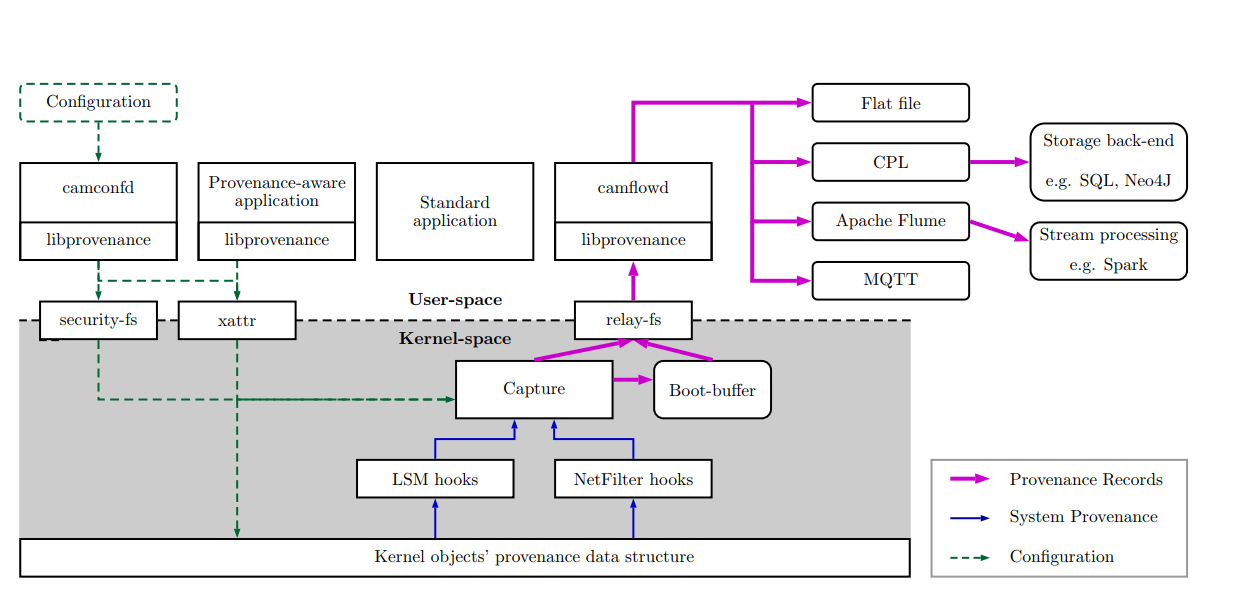
\includegraphics[width=0.7\linewidth]{camflow}
	\caption[Architecture overview]{Camflow architure}
	\label{fig:camflow}
\end{figure*}
\begin{figure}
	\centering
	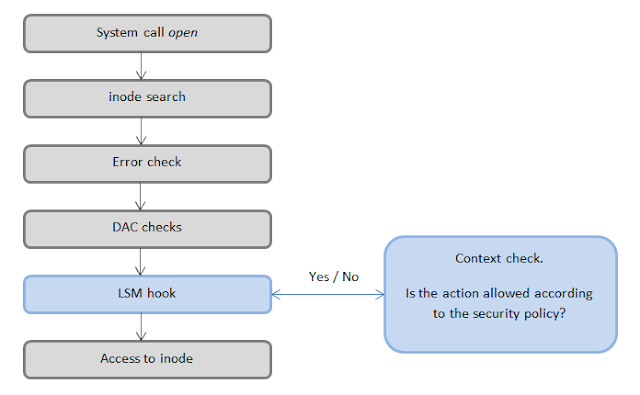
\includegraphics[width=0.7\linewidth]{LSM-hook}
	\caption[LSM hook]{LSM hook working for system call "open"}
	\label{fig:lsm-hook}
\end{figure}


\label{Introduction}
\section{LSMs and LSM hooks}
Though we have introduced what a Linux Security Module(LSM) means, we will discuss it in a little more detail. The Linux Security Module (LSM) framework provides a mechanism for various security checks to be hooked by new kernel extensions. The name “module” is a bit of a misnomer since these extensions are not actually loadable kernel modules. Instead, they are selectable at build-time via CONFIG\_DEFAULT\_SECURITY and can be overridden at boot-time via the "security=..." kernel command line argument, in the case where multiple LSMs were built into a given kernel.
\subsection{LSMs and policies}
The primary users of the LSM interface are Mandatory Access Control (MAC) extensions which provide a comprehensive security policy. Examples include SELinux, Smack, Tomoyo, and AppArmor. In addition to the larger MAC extensions, other extensions can be built using the LSM to provide specific changes to system operation when these tweaks are not available in the core functionality of Linux itself.
\subsection{Types of LSMs}
Without a specific LSM built into the kernel, the default LSM will be the Linux capabilities system. Most LSMs choose to extend the capabilities system, building their checks on top of the defined capability hooks.
\vskip 0.1in
The different types of Linux Security Modules are listed in Table 1. The entire list of the LSMs can be found by reading \textit{/sys/kernel/security/lsm}. The Table 1 reflects the order in which checks are made. The capability module is always first, followed by "minor" e.g. Yama) and then the one “major” module (e.g. SELinux) if there is one configured. This information will help us in understanding the next part of our research. 
\subsection{LSM Hooks}
In order to explain how a LSM hook works, we show an example in Fig 4. We take system call open as an example. We can see in Fig 4 that just before the kernel addresses an internal object, a check function provided by LSM is called. Hence, LSM allows the modules to understand wheather subject S is allowed to perform an action OP over kernel's internal object OBJ.


\begin{table}[ht]
	\caption{Linux Security Modules}
	\centering
	\begin{tabular}{c}
		\hline\hline 
		Different LSMs \\
		\hline
		AppArmor \\
		LoadPin  \\
		SELinux  \\
		Smack   \\
		TOMOYO \\
		Yama \\
	\end{tabular}	
\end{table}


\section{Modelling the system calls causing flows}
Analysis of programs aims verification of certain properties expected of them. Conventionally, there are two categories of anlysis, dynamic analysis and static analysis. Static analysis checks the properties on the souce code of the program, according to the declared semantics of the programming language, without the need to compile the program into machine language. 
The analysis proposed relies on the C compiler from the
Gnu Compilers Collection [23], used to compile the Linux
kernel.

\subsection{Control flow graphs}
The analysis technique we use if has been proposed by Georget et al. () for a subset of the system calls. It's a four step methodology which relies on the C compiler from the Gnu Compilers Collection(21). 

\begin{enumerate}
	\item The model designed by Georget to represent system calls and their execution paths does not describe the C source code. They instead use an internal representation called GIMPLE[]. 
	\item Each system call is represented by a control flow graph (CFG).
	\item The paths in these graphs model the execution paths in the program as defined by the classical graph theory[].
	\item The system calls are analysed one at a time. 
	\item Each system call contains multiple functions. These functions are inlined into the system calls to reduce the analysis to intra-procedural case. 
	\item Finally, in the CFGs, two kinds of nodes are marked: the nodes which correspond to the LSM hooks and the nodes which correspond to operation which generate the flows. 
	\end{enumerate}

\subsection{Constraints in modelling}
In the CFGs which we construct , a node is not a basic block but a simple GIMPLE instruction. The analysis methodology does not deal with all expressions and variables of the language. Another reason for the same is that usage of floating-point values is explicitly prohibited in the Linux code. Variables representing structures or unions are also not handled when they involve pointer arithmetic. Global or volatile variables are also not handled, since they can have an arbitrary value at any point in the execution. Ignoring some variables does not hinder the soundness of
our approach: less impossible paths might be detected as such but
we never declare as impossible a possible path. A path in the CFG is said to be impossible when any execution
that would follow it would enter in an impossible state. For example,
a path including two conditional branching with incompatible
conditions would require a Boolean expression to be both true and
false at the same time. 
\vskip 0.1in
There are powerful static analysers available such as Blast(24), available. However, for our need to ensure the complete mediation property, we don't need a framework which deals with complex types and data structures. Torvalds, creator and maintainer-in-chief of Linux has also developed a semantic analyzer for C called Sparse(27).
\vskip 0.1in
The mediation property which we have described in the previous section despite introducing the above mentioned constraints provides us with precise modelling.

\section{Static analysis on paths}
The goal of static analysis is to verify that information flow goes through a LSM hook or that it is impossible. In order to do so, we need to find the information flows for any CFG representing a system call.

\subsection{Verifying complete mediation}
We consider the set \textit{Paths} of all paths in a CFG.We introduce two particular subsets in this:(1) the set
Paths$_{flows}$  of paths starting at the initial node of the CFG and
ending at one node generating an information flow; and (2) the
set Paths$_{LSM}$  of paths having a node corresponding to a LSM
hook. The placement of the hooks would be obviously correct
if we could prove that Paths$_{flows}$ $\subseteq$ Paths$_{LSM}$ . However, as
we will see, this is not the case. Pf =  Paths$_{flows}$ \ Paths$_{LSM}$. The sets involved in the analysis are shown diagrammatically in Fig. 5.
represents the set of paths that may be problematic.
\vskip 0.1in
As explained earlier, some paths in Paths$_{flows}$  are actually
impossible, and therefore even if there are no LSM hooks
in them, they are not actually problematic. Recall that an
impossible path is a path that does not correspond to a possible
execution. The objective of our analysis is thus to verify that
P$_f$ $\subseteq$ I where I $\subseteq$ Paths is the set of impossible paths in
the CFG.
\vskip 0.1in
The property which we are looking to verify is the complete mediation property. Explaining the entire proof is out of scope of this paper. Hence, we state the entire property here.
\vskip 0.1in
\subsubsection[Property 1 (Complete Mediation)]{Property 1}\textit{(Complete Mediation)}
\vskip 0.2in
\textit{Complete mediation holds iff: P$_f$ $\subseteq$ I, i.e. all the execution
	paths that perform an information flow and are not controlled
	by the information flow monitor since they do not contain a
	LSM hook are impossible according to the static analysis.}
\begin{figure}
	\centering
	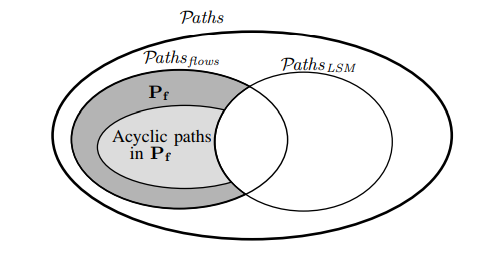
\includegraphics[width=0.7\linewidth]{Sets-involved}
	\caption[Sets involved in analysis]{Sets involved in analysis}
	\label{fig:sets-involved}
\end{figure}

\subsection{Soundness of proofs}
The soundness of our analysis is stated as follows.
\vskip 0.1in
\subsubsection{Theorem 1 }\textit{(Soundness)}
\vskip 0.1in

\textit{For each path p in a CFG, for all concrete configurations $\theta_1$
	and $\theta_2$, and all abstract configurations k$_1$ and k$_2$ such that
	$\theta_1$ $\rightarrow*_p$ $\theta_2$ and 
	k$_1$ $\rightarrow*p$ k$_2$, we have $\theta_1$ $\vDash$ k$_1$ $\Longrightarrow$ $\theta_2$ $\vDash$ k$_2$}
\vskip 0.2in
In simple words, according to the soundness property, executable paths are defined as the set of all paths p such that there exist two concrete configurations $\theta_1$ and $\theta_2$ such that $\theta_1$ $\rightarrow_p$ $\theta_2$. A transition may not exist from on configuration to another if, along the path p, there is an edge bearing a condition which is not verified by the memory state. e. The set of impossible paths is defined as the set of paths p for which
given any two abstract configurations k$_1$ and k$_2$, if k$_1$ $\rightarrow_p*$ k$_2$, then
$\nvDash$ k$_2$. In other words, there is no satisfiable configuration that can
result from the analysis of path p. The following proposition is an
immediate consequence of the previous one.
\vskip 0.2in

\subsubsection{Theorem 2 }\textit{(Executable vs Impossible paths)}
\vskip 0.1in
\textit{The sets of
	executable paths and impossible paths are disjoint.}

\subsection{Implementation and results}
The static analysis is run during the compilation itself. To this effect, we use the plug-ins developed by Georget et al. We also followed the same methodology as proposed by Georget et al. in the previous kernel version 4.3. We performed the experimentation for kernel version 4.20 which is the last stable release as of now. 
\vskip 0.2in
We use a plugin developed by Geroget () for GCC version 4.8.  This plugin is
inserted into the compilation process, when the code is in GIMPLE
form. We chose to place the plugin as late as possible in the compilation process, just before GCC abandons the graph intermediate
representation, in order to benefit the most from optimizations
and to work on a code as simple as possible. This allows us to do
the assumptions we presented in the previous sections, such as
the particular properties of loops. The representation we dump is
broken down to very elementary pieces. The code we handle is in
three-addresses mode, which has the effect that all complex boolean
conditions that could exist in the original code base are already
broken down in the appropriate number of binary decision nodes
and branching. We also leverage as much as possible the compiler.
For example, we rely on it to identify the loops in the CFG, to know
the precise typing information of variables, and to run the points-to
analysis on pointers. The latter is already implemented because it
is used for several optimizations passes by GCC. Finally, the careful
use of inlining and the fact that GCC applies some optimizations
on the code actually limits the path explosion. We make use of the tools available on the kayrebt website (31).

In order to do so, we first look at the system calls difference between kernel version 4.3 and 4.20. In total we identify 460 system calls in the stable release 4.20. But from the observation, we can also notice that not all system calls are capable of generating flows. Understanding the difference between the system calls between different kernel versions, itself is a separate study. The previous study was done by Hauser (32) for the kernel version 4.7 for his doctoral thesis. New system calls are added and used as per the applications requirements. 
\vskip 0.2in
Prior to running analysis,we first need to place a special annotations on tplaces in the code of system calls where information flows are performed. When the analysis is run on a system call, for each
annotated places, a subgraph of the CFG built by GCC is considered:
the subgraph of paths starting from the node representing the entry
of the system call and going to the information flow node that
do not pass through any LSM hook. These paths are the set P$_f$
.
For each path, we start with an empty abstract configuration and
we update the configuration as we go along the path as per the
transition rules of the abstract semantics. The satisfiability of the
abstract configuration is tested by Yices [5], a SAT-solver equipped
with a decidable subset of the classic theory of integers. If the
constraint solver declares the set of constraints unsatisfiable then
we declare the path impossible.
\vskip 0.2in
In order to understand and visualize the information flows, we use the tools available on http://kayrebt.gforge.inria.fr/. We categorize the flows into two types discrete flow and continuous flow as shown in the Table 2, 3 and 4. Table 2 shows a summary of the discrete flows for the different types of system calls. We have similar flows recorded for the write, send, receive system calls. Table 3 shows the system calls which were updates in the kernel version 4.20. However, Georget did a similar analysis and found the missing LSM hooks for 29 system calls which were updated from kernel version 3.2 to 4.3. Table 4 lists the system calls from version 4.3 to 4.20 whose information flows which are discrete do not trigger all LSM hooks. Table 5 shows system calls added from version 4.3 to 4.20 which do not trigger all LSM hooks when called. These system calls have continuous flows. This means that the flow is from both sides, the file to the memory and vice versa. However, we notice that the LSM hook is triggered only once during the exchange.

\begin{table}[ht]
	\caption{Read system calls}
	\centering
	\begin{tabular}{c c}
		\hline\hline 
	System calls & Discrete flow  \\
		\hline
		read & File $\rightarrow$ memory of the calling process \\
			readv & File $\rightarrow$ memory of the calling process \\
				preadv & File $\rightarrow$ memory of the calling process \\
					pread64 & File $\rightarrow$ memory of the calling process \\

	\end{tabular}	
\end{table}


\begin{table}[ht]
	\caption{Updated system calls in version 4.20}
	\centering
	\begin{tabular}{c c}
		\hline\hline 
		System calls & Discrete flow  \\
		\hline
		vmsplice. & Memory of the calling process $\rightarrow$ tube \\
		 & tube $\rightarrow$ memory of the calling process \\
		process\_vm\_readv & Memory of another process  \\
	 & $\rightarrow$ memory of the calling process \\
	 	process\_vm\_writev & Memory of another process  \\
	 & $\rightarrow$ memory of the calling process \\
		
	\end{tabular}	
\end{table}

\begin{table}[ht]
	\caption{Updated system calls in version 4.20 which don't trigger LSM hooks but have discrete flows.}
	\centering
	\begin{tabular}{c c}
		\hline\hline 
		System calls & Discrete flow  \\
		\hline
		migrate\_pages & Memory of another process  \\
		& $\rightarrow$ memory of the calling process \\
		move\_pages & Memory of another process  \\
		& $\rightarrow$ memory of the calling process \\
		
		
	\end{tabular}	
\end{table}

\begin{table}[ht]
	\caption{Updated system calls in version 4.20 which don't trigger LSM hooks but have discrete flows.}
	\centering
	\begin{tabular}{c c}
		\hline\hline 
		System calls & continuous flow  \\
		\hline
	
		mmap\_pgoff. & Regular file or device  \\
		& $\leftrightarrow$ memory of the current process \\
		& regular file or device  \\
		& $\rightarrow$ memory of the current process \\
		
	\end{tabular}	
\end{table}


